\documentclass[a4paper,14pt]{extreport}
	\usepackage[left=1.5cm,right=1.5cm,
	    top=1.5cm,bottom=2cm,bindingoffset=0cm]{geometry}
	\usepackage{scrextend}
	\usepackage[T1,T2A]{fontenc}
	\usepackage[utf8]{inputenc}
	\usepackage[english,russian,ukrainian]{babel}
	\usepackage{tabularx}
	\linespread{1.5}
	\usepackage{amssymb}
	\usepackage{fp}
	\usepackage{color}
	\usepackage{amsmath}
	\usepackage{mathrsfs}
	\usepackage{listings}
	\usepackage{graphicx}
	\graphicspath{ {./images/} }
	\usepackage{lipsum}
	\usepackage{xcolor}
	\usepackage{multirow}
	%\usepackage[table,xcdraw]{xcolor}
	\usepackage{hyperref}
	\usepackage{tcolorbox}
	\usepackage{tikz}
	\usepackage[framemethod=TikZ]{mdframed}
	\usepackage{wrapfig,boxedminipage,lipsum}
	\mdfdefinestyle{MyFrame}{%
	linecolor=blue,outerlinewidth=2pt,roundcorner=20pt,innertopmargin=\baselineskip,innerbottommargin=\baselineskip,innerrightmargin=20pt,innerleftmargin=20pt,backgroundcolor=gray!50!white}
	 \usepackage{csvsimple}
	 \usepackage{supertabular}
	\usepackage{pdflscape}
	\usepackage{fancyvrb}
	%\usepackage{comment}
	\definecolor{ggreen}{rgb}{0.4,1,0}
	\definecolor{rred}{rgb}{1,0.1,0.1}
	\definecolor{aquamarine}{rgb}{0.5, 1.0, 0.83}
	\definecolor{amber}{rgb}{1.0, 0.75, 0.0}
	\definecolor{babyblue}{rgb}{0.54, 0.81, 0.94}
	\definecolor{buff}{rgb}{0.94, 0.86, 0.51}
	\definecolor{internationalorange}{rgb}{1.0, 0.31, 0.0}
	\definecolor{lightmauve}{rgb}{0.86, 0.82, 1.0}
	\definecolor{mediumaquamarine}{rgb}{0.4, 0.8, 0.67}
	\usepackage{array,tabularx}
	\usepackage{colortbl}
	
	\usepackage{varwidth}
	\tcbuselibrary{skins}
	\usepackage{fancybox}

	\usetikzlibrary{calc}
	\makeatletter
	\newlength{\mylength}
	\xdef\CircleFactor{1.1}
	\setlength\mylength{\dimexpr\f@size pt}
	\newsavebox{\mybox}
	\newcommand*\circled[2][draw=blue]{\savebox\mybox{\vbox{\vphantom{WL1/}#1}}\setlength\mylength{\dimexpr\CircleFactor\dimexpr\ht\mybox+\dp\mybox\relax\relax}\tikzset{mystyle/.style={circle,#1,minimum height={\mylength}}}
	\tikz[baseline=(char.base)]
	\node[mystyle] (char) {#2};}
	\makeatother
	\usepackage{pgfplots}
    \pgfplotsset{compat=1.9}


	\usepackage{float}
	\usepackage{wrapfig}
	\usepackage{framed}
	%for nice Code{
	\lstdefinestyle{customc}{
	  belowcaptionskip=1\baselineskip,
	  breaklines=true,
	  frame=L,
	  xleftmargin=\parindent,
	  language=C,
	  showstringspaces=false,
	  basicstyle=\small\ttfamily,
	  keywordstyle=\bfseries\color{green!40!black},
	  commentstyle=\itshape\color{purple!40!black},
	  identifierstyle=\color{blue},
	  stringstyle=\color{orange},
	}
	\lstset{escapechar=@,style=customc}
	\usepackage{enumitem}

	% Цвета для гиперссылок
  \definecolor{linkcolor}{rgb}{1.0, 0.22, 0.0}% цвет ссылок
  \definecolor{urlcolor}{rgb}{0.4, 1.0, 0.0}% цвет гиперссылок
  \hypersetup{pdfstartview=FitH,  linkcolor=linkcolor,urlcolor=urlcolor,citecolor=red, colorlinks=true}
%}


\begin{document}
\newtcbox{\xmybox}[1][red]{on line, arc=7pt,colback=#1!10!white,colframe=#1!50!black, before upper={\rule[-3pt]{0pt}{10pt}},boxrule=1pt, boxsep=0pt,left=6pt,right=6pt,top=2pt,bottom=2pt}
\pagecolor{white}
\begin{titlepage}
	\begin{center}
	\large
	Національний технічний університет України \\ "Київський політехнічний інститут імені Ігоря Сікорського"


	Факультет Електроніки

	Кафедра мікроелектроніки
	\vfill

	\textsc{ЗВІТ}\\

	{\Large Про виконання лабораторної роботи №1\\
	з дисципліни: «Схемотехніка-2. Цифрова схемотехніка»\\[1cm]

	ЕЛЕКТРОННІ КЛЮЧІ


	}
	\bigskip
	\end{center}
	\vfill

	\newlength{\ML}
	\settowidth{\ML}{«\underline{\hspace{0.4cm}}» \underline{\hspace{2cm}}}
	\hfill
	\begin{minipage}{1\textwidth}
	Виконавець:\\
	Студент 4-го курсу \hspace{4cm} $\underset{\text{(підпис)}}{\underline{\hspace{0.2\textwidth}}}$  \hspace{1cm}А.\,С.~Мнацаканов\\


	Перевірила: \hspace{5.9cm} $\underset{\text{(підпис)}}{\underline{\hspace{0.2\textwidth}}}$  \hspace{1cm}Г.\,С.~Порева\\

	\end{minipage}

	\vfill

	\begin{center}
	2021
	\end{center}
\end{titlepage}





\begin{center}
\fbox{ПЕРЕМИКАЧ НАПРУГИ НА БІПОЛЯРНОМУ ТРАНЗИСТОРІ}

\end{center}

\begin{figure}[h]
	\center{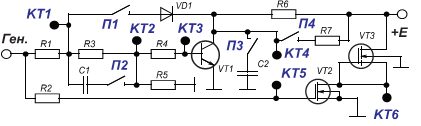
\includegraphics[width=0.7\linewidth]{1.png}}
	\caption{Перемикачі напруги на біполярному транзисторі та на МДН-транзисторі з індукованим каналом.}
	\label{ris1}
\end{figure}

\textbf{Мета роботи} - дослідити статичні та динамічні характеристики
електронного ключа на біполярному транзисторі (БТ) та схемні прийоми
покращення параметрів цього типу електронного ключа.

\begin{figure}[h]
	\center{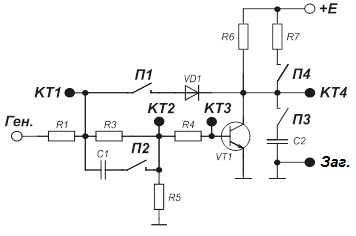
\includegraphics[width=0.5\linewidth]{2.png}}
	\caption{Перемикачі напруги на біполярному транзисторі.}
	\label{ris2}
\end{figure}


\begin{center}
\textbf{Робоче завдання}
\end{center}
Встановити лабораторний стенд «ИМПУЛЬС-М» в режим «ЛАБ-1» за допомогою перемикача лабораторних робіт, який знаходиться на задній панелі стенда. 
Ввімкнути кнопку «СЕТЬ».\\

\textbf{I}. За допомогою генератора Ген. подати на вхід ключа позитивний прямокутний імпульс тривалістю 200 мкс з частотою 1кГц. 
Зняти й побудувати передавальну характеристику. За допомогою цієї характеристики визначити статичні параметри ключа: $U_2^0$та $U_1^2$. Для цього потрібно змінювати амплітуду вхідного імпульсу $U_1$та визначати відповідну амплітуду сигналу на виході $U_2$. 
Виконати вимірювання для наступних режимів роботи:
\begin{enumerate}
	\item Схемі із відключеними компонентами: діодом , конденсаторами  і  та опором  (П1-П4 ). 
    \item Схема із підключеним діодом  (натиснути П1).
    \item Схема із підключеним конденсатором  (натиснути П2).
    \item Схема із підключеним резистором  (натиснути П4).
\end{enumerate}
 
		Результати зазначений вимірювань занести в табл.\ref{tab1} та відобразити на рис. \ref{ris3}.
\begin{table}[h]%1
	\begin{center}
	\begin{large}
	\caption{Результати вимірювання передавальної характеристики  перемикача напруги на біполярному транзисторі для різних модифікацій схеми.}
		\begin{tabular}{|c|c|c|c|c|c|c|c|}
			\hline
			$U_1, B$                                                             & 1,8 & 2,4 & 2,6 & 2,8 & 2,9 & 3 & 3,2   \\ \hline
			\begin{tabular}[c]{@{}c@{}}$U_2, B$\\ (П1-П4$\uparrow$)\end{tabular} & 5 & 4,8 & 4 & 2 & 1 & 0,5 & 0,5   \\ \hline
			\begin{tabular}[c]{@{}c@{}}$U_2, B$\\ для $VD_1$ (П1$\downarrow$)\end{tabular} & 5 & 4,8 & 4 & 2 & 2,5 & 2,5 & 2  \\ \hline
			\begin{tabular}[c]{@{}c@{}}$U_2, B$\\ для $C_1$ (П2 $\downarrow$)\end{tabular} & 5 & 4,8 & 4 & 2 & 1 & 0,5 & 0,4   \\ \hline
			\begin{tabular}[c]{@{}c@{}}$U_2, B$\\ для $R_7$ (П4$\downarrow$)\end{tabular} & 5 & 4,9 & 4,5 & 3,8 & 3 & 0,5 & 0,5   \\ \hline
		\end{tabular}
	\end{large}
	\end{center}
	
	\label{tab1}
\end{table}

 
\begin{figure}[h]
	\center{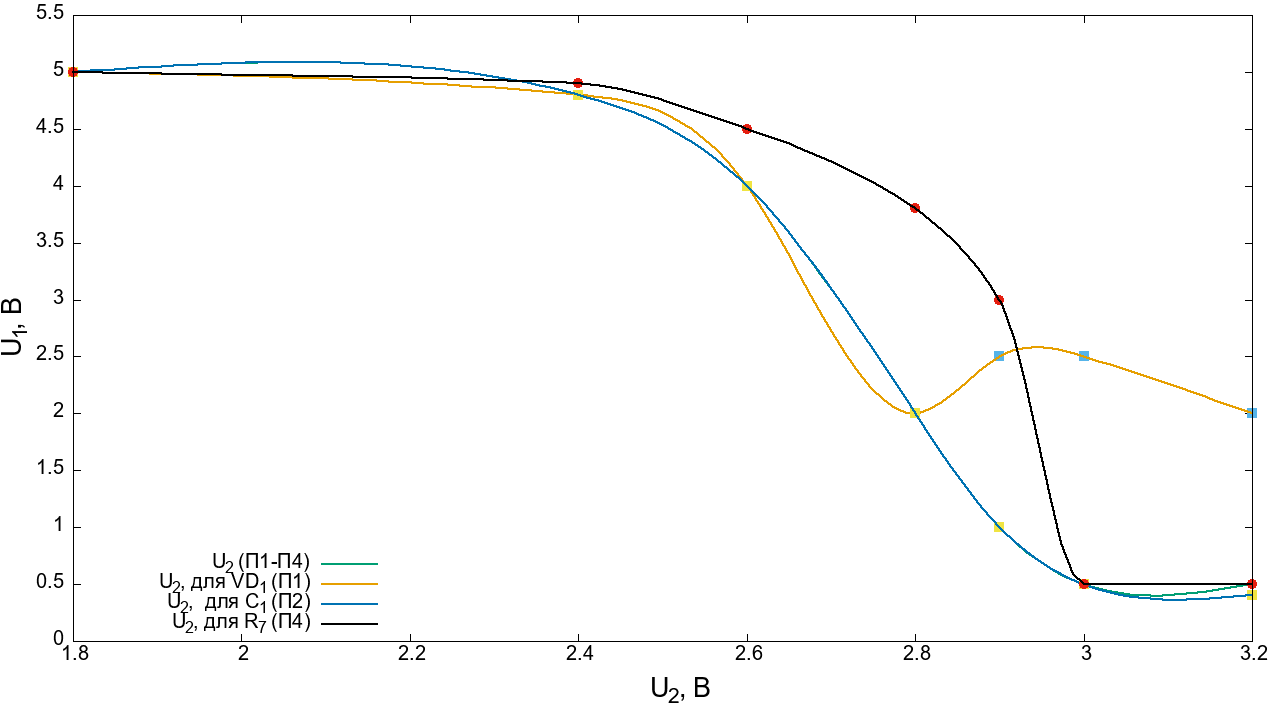
\includegraphics[width=1\linewidth]{fortab1.png}}
	\caption{Результати вимірювання передавальної характеристики $U_2 = f(U_1)$
перемикача напруги на біполярному транзисторі для різних модифікацій схеми.}
	\label{ris3}
\end{figure}

\textbf{II} За допомогою генератора Ген. подати на вхід ключа позитивний
прямокутний імпульс із амплітудою $U_1^1$ = 5 В, тривалістю $t_{\text{вх}}$ = 40 мкс та частотою $f_{\text{вх}}$ = 10кГц.\\
При вимірюваннях потрібно використати зовнішню синхронізацію осцилографа від генератора прямокутних імпульсів.\\
Визначити перехідну характеристику $U_2(t)$ транзисторного ключа при
його вмиканні та розмиканні. З урахуванням масштабів замалювати діаграми
вхідного $U_1(t)$ та вихідного $U_2(t)$ імпульсів за шаблоном, наведеним на рис.\ref{ris4}. За допомогою осцилографа визначити динамічні параметри ключа:

тривалість фронтів вихідного сигналу $t^{10}_\text{ф}$, $t^{01}_\text{ф}$ та тривалість затримок поширення
вихідного сигналу відносно вхідного $t^{10}_\text{зп}$, $t^{01}_\text{зп}$. При
виконанні вимірювань осцилограф потрібно налаштувати таким чином, щоб
масштаб часу дозволяв визначити ці параметри максимально точно.
Виконати вимірювання для наступних режимів роботи:
\begin{enumerate}
	\item Схемі із відключеними компонентами: діодом $VD_1$, конденсаторами $C_1 $і $C_2$ та опором $R_7$ (П1-П4).
    \item Схема із підключеним діодом 1VD (натиснути П1).
    \item Схема із підключеним конденсатором $C_1$ (натиснути П2).
    \item Схема із підключеним конденсатором $C_2$ (натиснути П3).
    \item Схема із підключеним резистором $R_7$ (натиснути П4).
\end{enumerate}


\begin{table}[h]
	\begin{center}
	\caption{Результати вимірювання фронтів вихідного сигналу $t^{10}_\text{ф}$, $t^{01}_\text{ф}$ 	затримок поширення вихідного сигналу відносно вхідного $t^{10}_\text{зп}$, мкс  $t^{01}_\text{зп}$ перемикача
	напруги на біполярному транзисторі для різних модифікацій схеми.}
	\begin{tabular}{|c|c|c|c|c|}
		\hline
		    &$t^{10}_\text{ф}$, мкс  &$t^{01}_\text{ф}$, мкс  & $t^{10}_\text{зп}$, мкс & $t^{01}_\text{зп}$, мкс \\ \hline
		\begin{tabular}[c]{@{}c@{}}$R_6$\\ (П1-П4)\end{tabular} &0,12  & 0,4 &0,4  &0,4  \\ \hline
		\begin{tabular}[c]{@{}c@{}}$VD_1$\\ (П1)\end{tabular}   &0,018  &0,18  &0,4  &0,35  \\ \hline
		(П2)                                                    & 0,008 &0,1  &0,14  &0,2  \\ \hline
		\begin{tabular}[c]{@{}c@{}}$R_7$\\ (П4)\end{tabular}    &0,016  &0,07  &0,42  &0,4  \\ \hline
		\begin{tabular}[c]{@{}c@{}}$C_3$\\ (П3)\end{tabular}      &0,024  & 0,25 &0,5  &0,48  \\ \hline
	\end{tabular}
	
	\label{tab2}
	\end{center}
\end{table}


%----------------------------------------------------------
\begin{figure}[h]
	\center{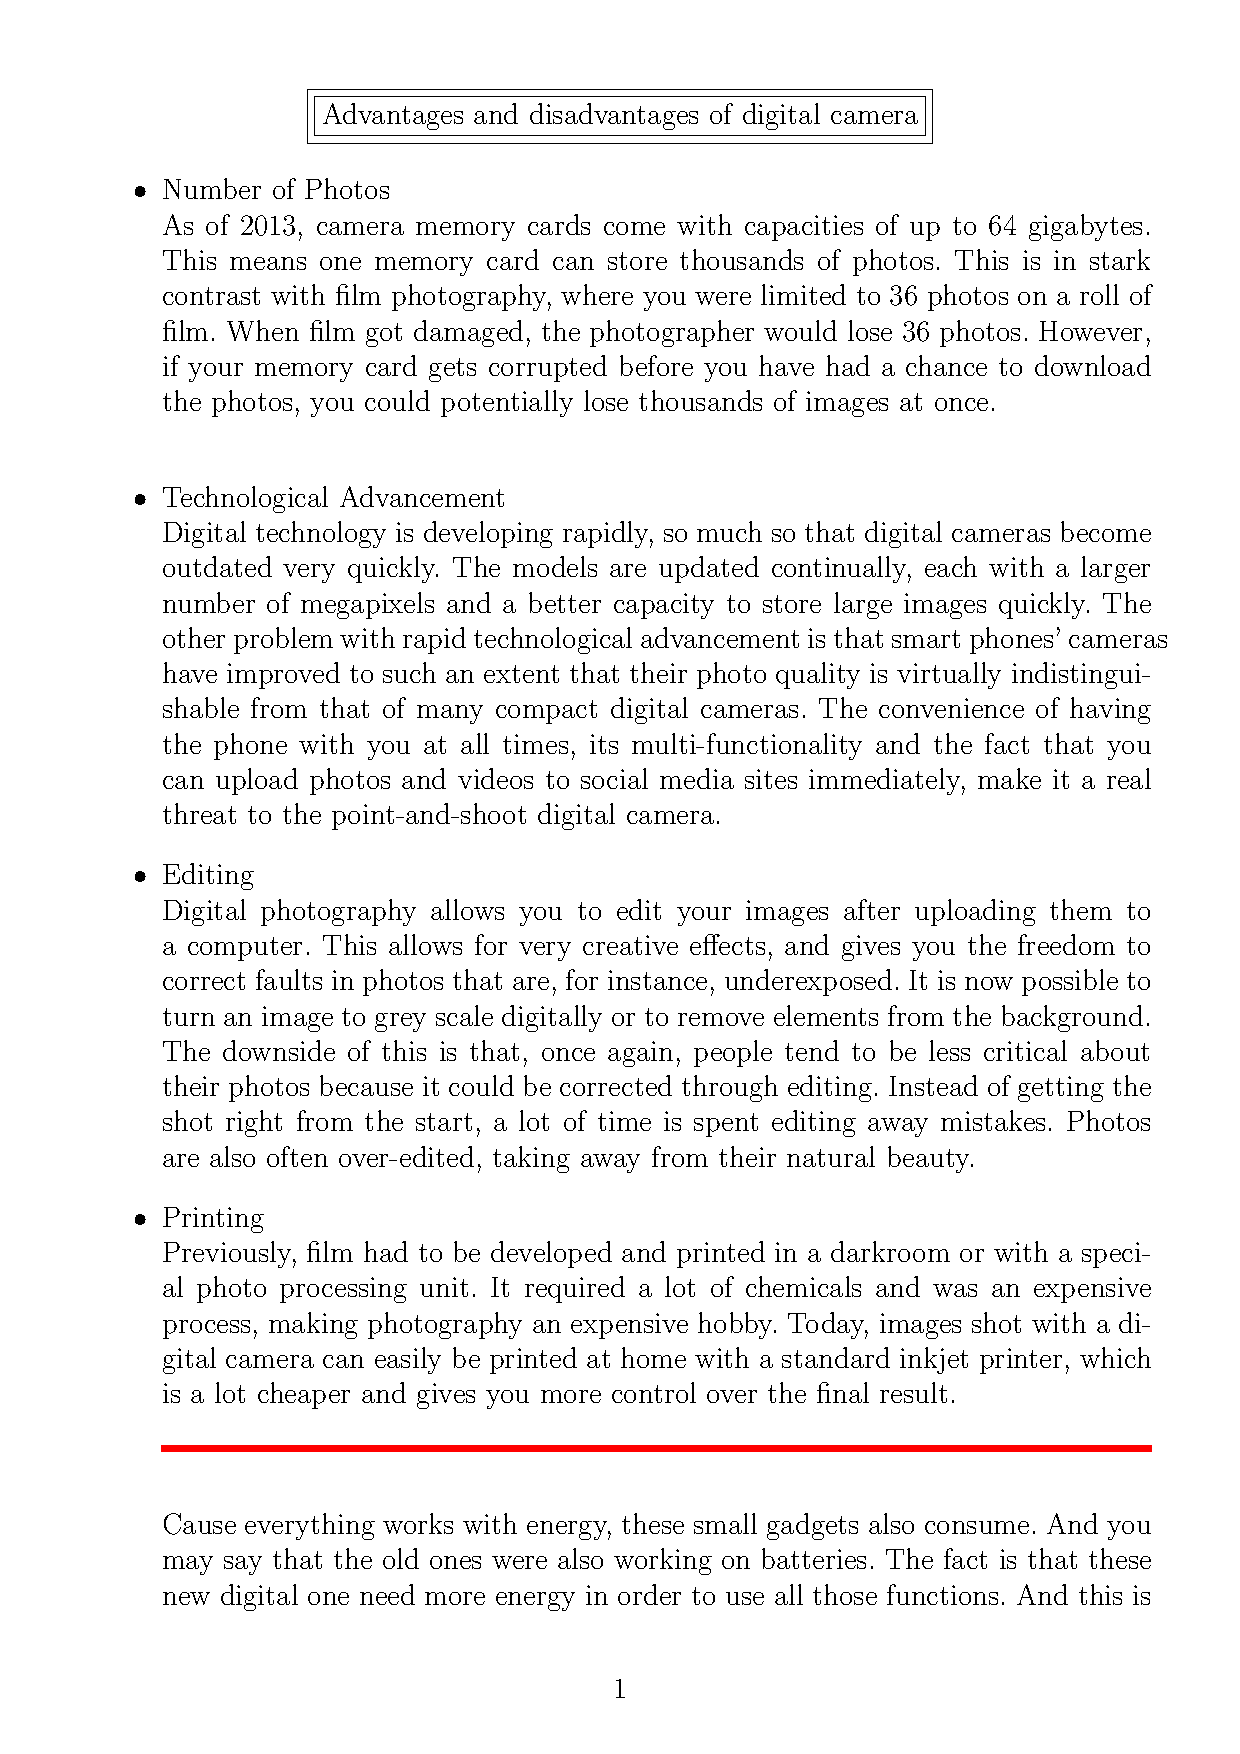
\includegraphics[width=1\linewidth]{4.pdf}}
	\caption{Залежності вхідного та вихідних сигналі від часу перемикача напруги на біполярному транзисторі для різних модифікацій схеми.}
	\label{ris4}
\end{figure}
\begin{center}
\fbox{ПЕРЕМИКАЧ НАПРУГИ НА МДН – ТРАНЗИСТОРІ} \fbox{С ІНДУКОВАНИМ КАНАЛОМ}
\end{center}

\textbf{Мета роботи} - дослідити статичні і динамічні параметри перемикача напруги на МДН - транзисторі з індукованим каналом.

\begin{figure}[h]
	\center{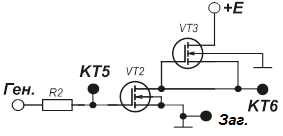
\includegraphics[width=0.6\linewidth]{5.png}}
	\caption{Перемикачі напруги на МДН-транзисторі з індукованим каналом.}
	\label{ris5}
\end{figure}


\begin{center}
\textbf{Робоче завдання}
\end{center}

\textbf{I}. За допомогою генератора Ген. подати на вхід ключа позитивний прямокутний імпульс тривалістю $t_{\text{вх}}$=200мкс з частотою $f_{\text{вх}}$=1 кГц. \\

Зняти й побудувати передавальну характеристику . За допомогою цієї характеристики визначити статичні параметри ключа:  $U_2^0$ та $U_2^1$. Для цього потрібно змінювати амплітуду вхідного імпульсу $U_1$ та визначати відповідну амплітуду сигналу на виході $U_2$. \\

Результати вимірювань звести до табл.\ref{tab3}  та відобразити за шаблоном, наведеним на рис.\ref{ris3}.

\begin{table}[h!]
	\begin{center}
	\caption{Результати вимірювання передавальної характеристики $U_2 = f(U_1)$ перемикача напруги на МДН-транзисторі з індукованим каналом}
		\begin{tabular}{|c|c|c|c|c|c|c|c|}
			\hline
			$U_1$, B & 2 & 2,2 & 2,4 & 2,5 & 2,6 & 2,61 & 2,7 \\ \hline
			$U_2$, B & 5 & 4,8 & 3 & 2 & 0,9 & 0,2 & 0,1 \\ \hline
		\end{tabular}
	
		
		\label{tab3}

	\end{center}
\end{table}

 
\begin{figure}[h!]
	\center{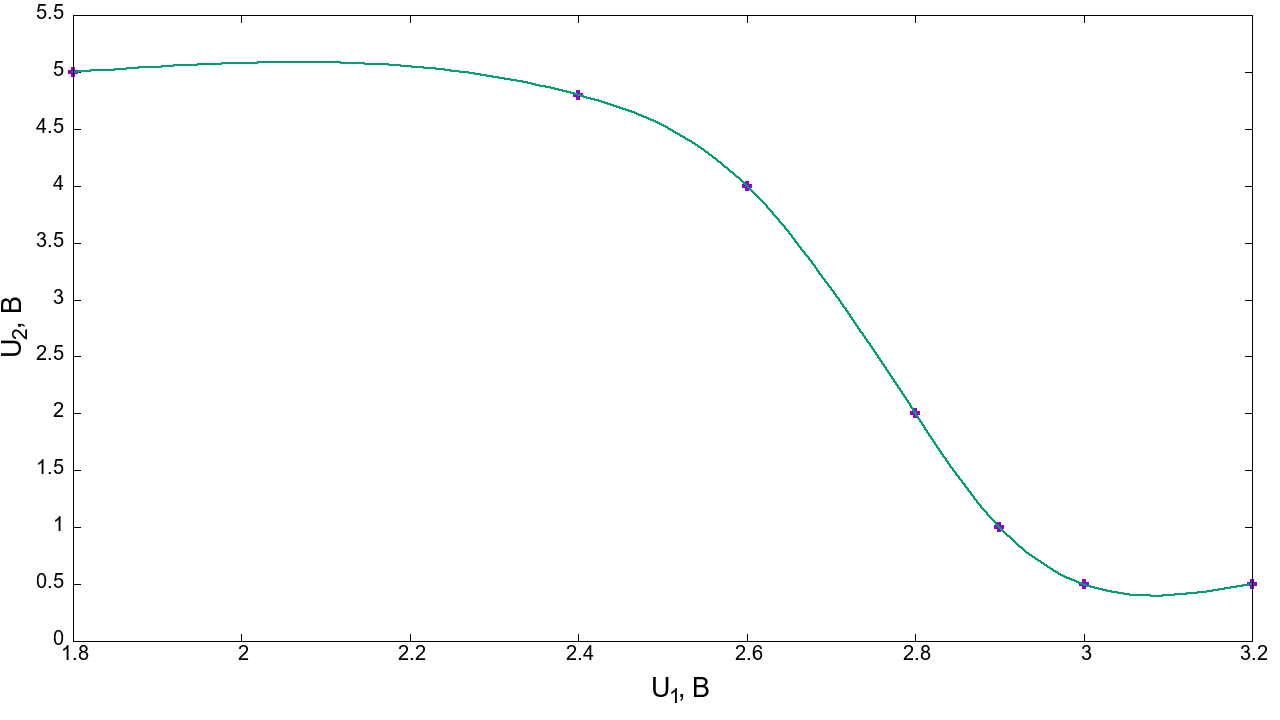
\includegraphics[width=1\linewidth]{fortab2.png}}
	\caption{Передавальна характеристика $U_2 = f(U_1)$ перемикача напруги на МДН-транзисторі з індукованим каналом.}
	\label{ris3}
\end{figure}

\textbf{II} За допомогою генератора Ген. подати на вхід ключа позитивний прямокутний імпульс із амплітудою $U_1^1$=5В, тривалістю $t_{\text{вх}}$=40мкс та частотою $f_{\text{вх}}$=10кГц.
При вимірюваннях потрібно використати зовнішню синхронізацію осцилографа від генератора прямокутних імпульсів.
Визначити перехідну характеристику $U_2(t)$ транзисторного ключа при його вмиканні та розмиканні. З урахуванням масштабів замалювати діаграми вхідного $U_1(t)$  та вихідного $U_2(t)$  імпульсів за шаблоном. За допомогою осцилографа визначити динамічні параметри ключа: тривалість фронтів вихідного сигналу $t_{\text{ф}}^{10}$ , $t_{\text{ф}}^{01}$ та тривалість затримок поширення вихідного сигналу відносно вхідного $t_{\text{зв}}^{10}$, $t_{\text{зв}}^{01}$. При виконанні вимірювань осцилограф потрібно налаштувати таким чином, щоб масштаб часу дозволяв визначити ці параметри максимально точно.

\begin{table}[h]
	\begin{center}
	\caption{Результати вимірювання фронтів вихідного сигналу ,  та затримок поширення вихідного сигналу відносно вхідного ,  перемикача напруги на МДН-транзисторі з індукованим каналом.}
		\begin{tabular}{|c|c|c|c|}
			\hline
			 $t_{\text{ф}}^{10}$ , мкс& $t_{\text{ф}}^{01}$ , мкс &$t_{\text{зв}}^{10}$ , мкс  & $t_{\text{зв}}^{01}$ , мкс \\ \hline
			 0,75& 0,5 &  1& 1 \\ \hline
		\end{tabular}
		
		\label{tab4}
	\end{center}
\end{table}





\begin{figure}[h!]
	\center{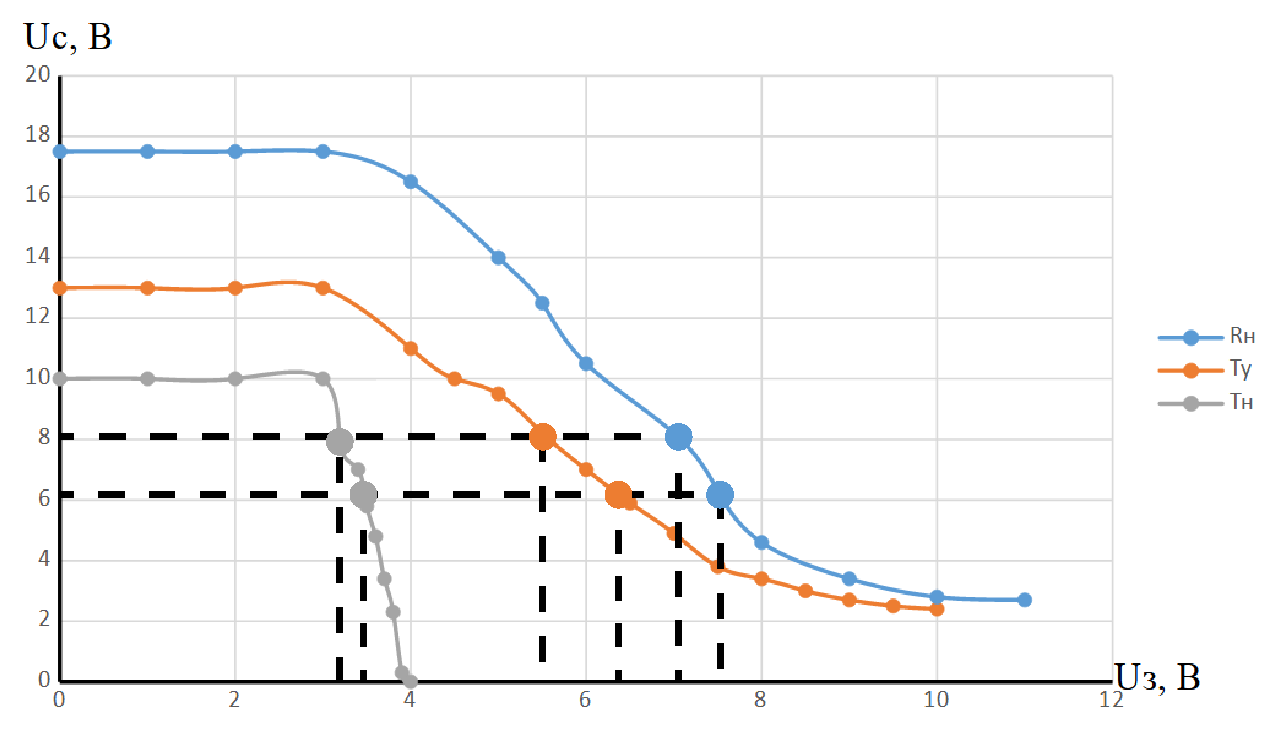
\includegraphics[width=0.8\linewidth]{6.pdf}}
	\caption{Залежності вхідного та вихідних сигналі від часу перемикача напруги на МДН-транзисторі з 
	індукованим каналом.}
	\label{ris3}
\end{figure}


\clearpage 
\newpage
\begin{center}
\textbf{\fbox{Висновок}}
\end{center}
Аналізуючи дані отримані в ході лабораторної роботи для 
бiполярного транзистора можна стверджувати, що по-перше, за допомогою $C_1$ транзистор  переводить  у вiдкритий стан набагато швидше порівняно з иншими компонентами, а також затримка вiдносно  вхiдного сигналу теж стає меншою, до тогог ж при ввiмкненнi навантажувальної ємностi, час усталення всіх перехiдних процесiв та затримка мiж вхiдним та вихiдним сигналом стає доволi значною. По-друге, було також помічено при обробці результатів, що $R_7$, який паралельно пiдключений до резистора $R_6$, забезпечив \textbf{найшвидше} закриття резистора.\\


В схемі на польовому транзисторі показує присутні незначні перехiднi процеси, проте вони все ж таки присутні.









\end{document}